% !TEX root =  master.tex
\chapter{Entwurf}\label{entwurf}
	\section[Design Entwurf]{Design Entwurf {\hfill \normalsize Milena Zahn}}\label{design}
		\begin{figure}[H]
			\centering 
			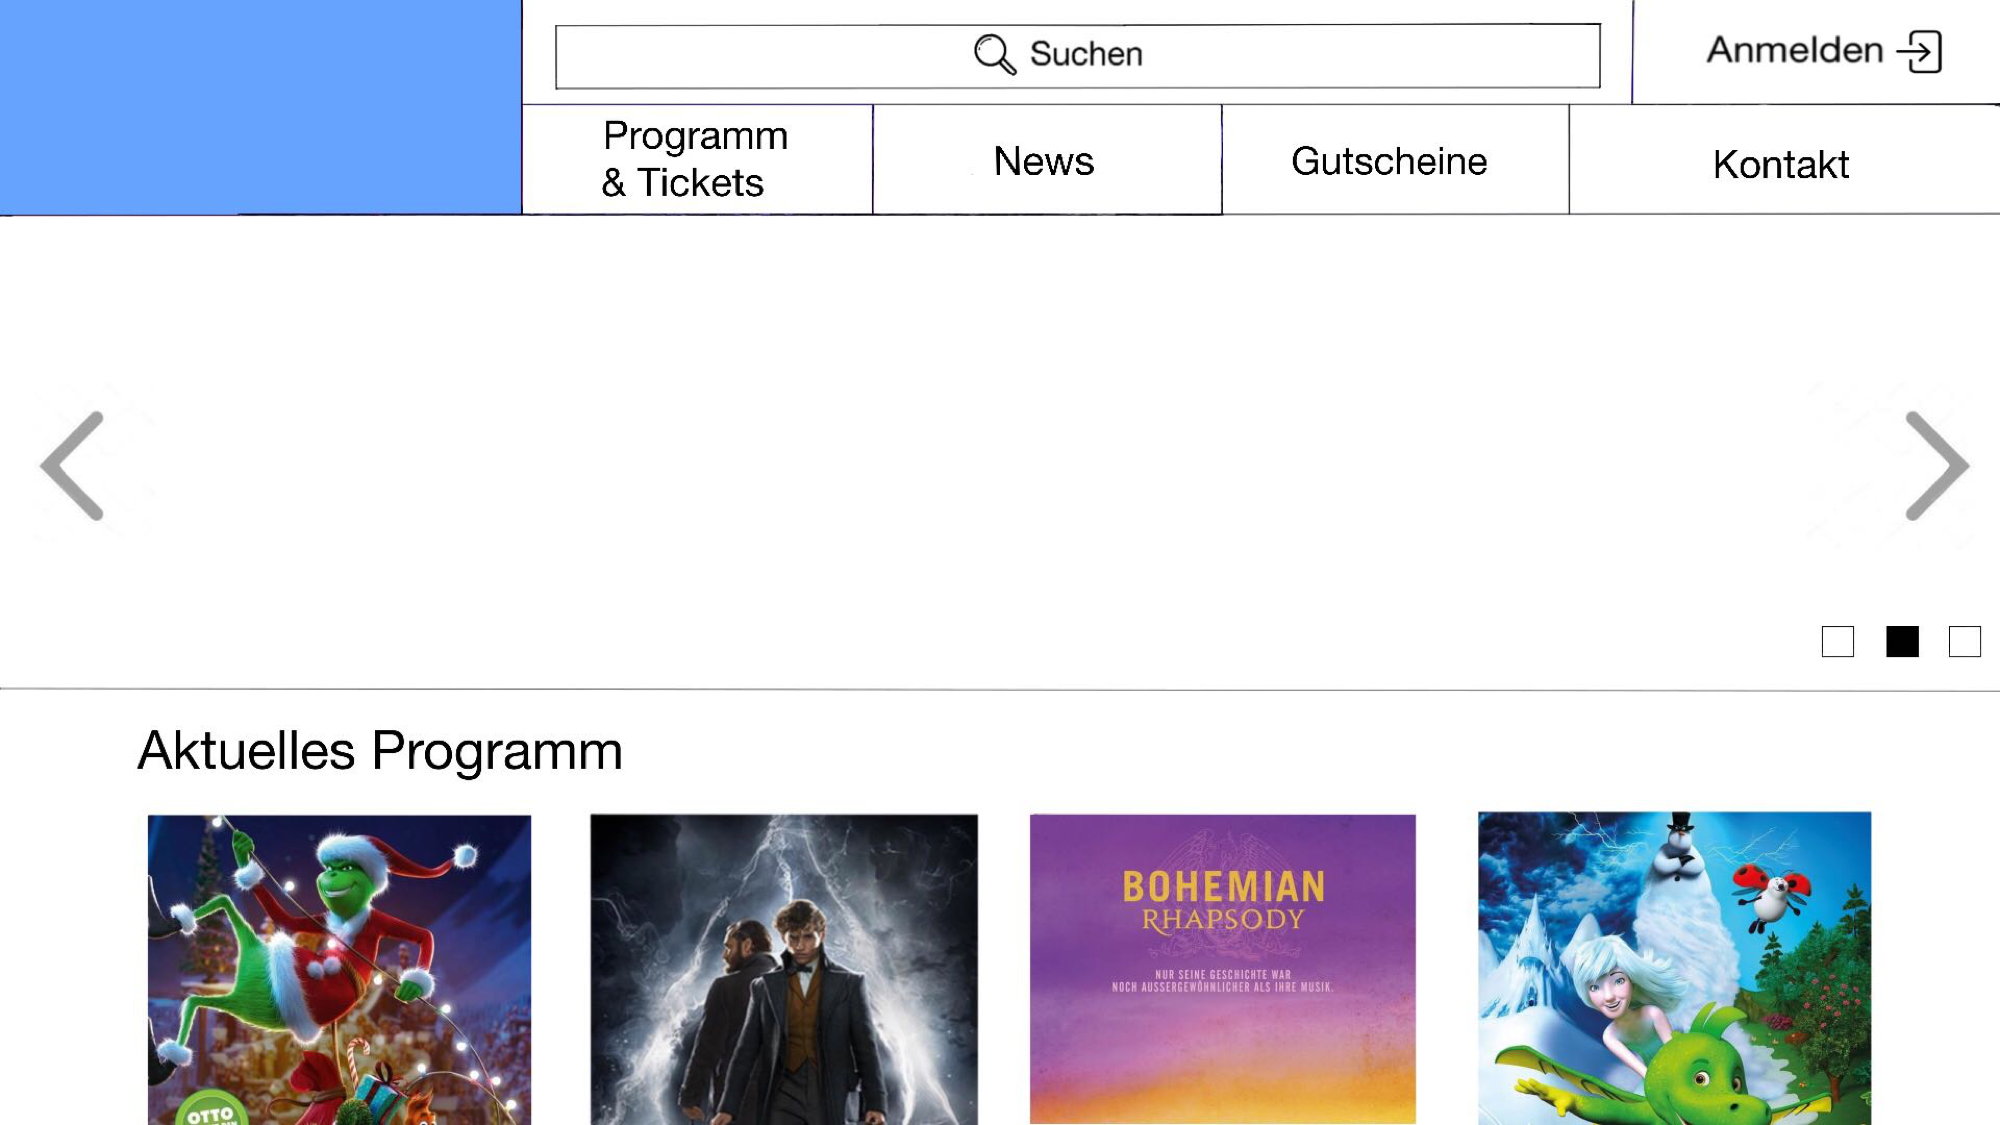
\includegraphics[width=14cm]{img/mockUp1.png}
			\captionsetup{format=hang}
			\caption[Mockup Startseite]{\label{fig:mockUpStartseite} Mockup Startseite }
		\end{figure}
		\begin{figure}[H]
			\centering 
			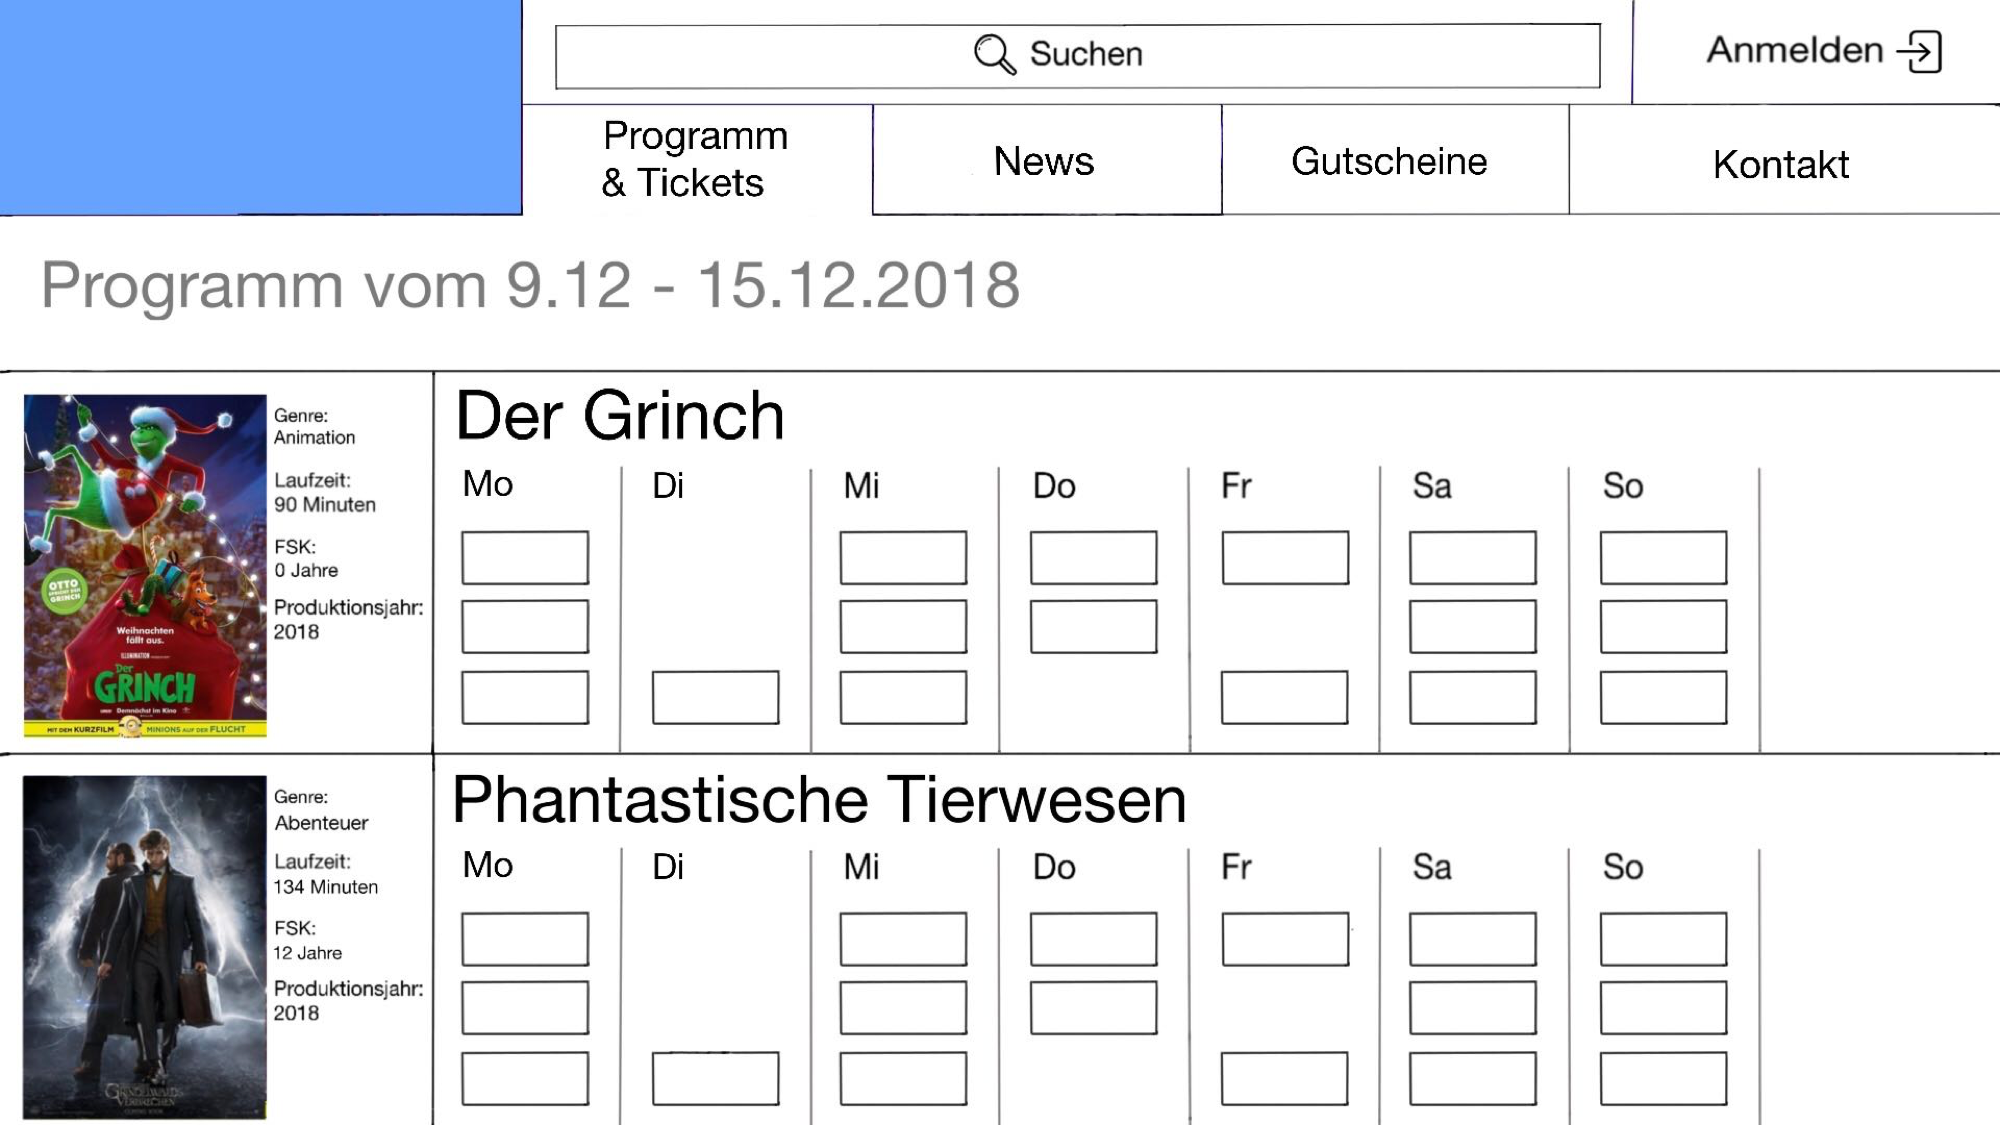
\includegraphics[width=14cm]{img/mockUp2.png}
			\captionsetup{format=hang}
			\caption[Mockup Programm]{\label{fig:mockUpProgramm} Mockup Programm }
		\end{figure}
		\begin{figure}[H]
			\centering 
			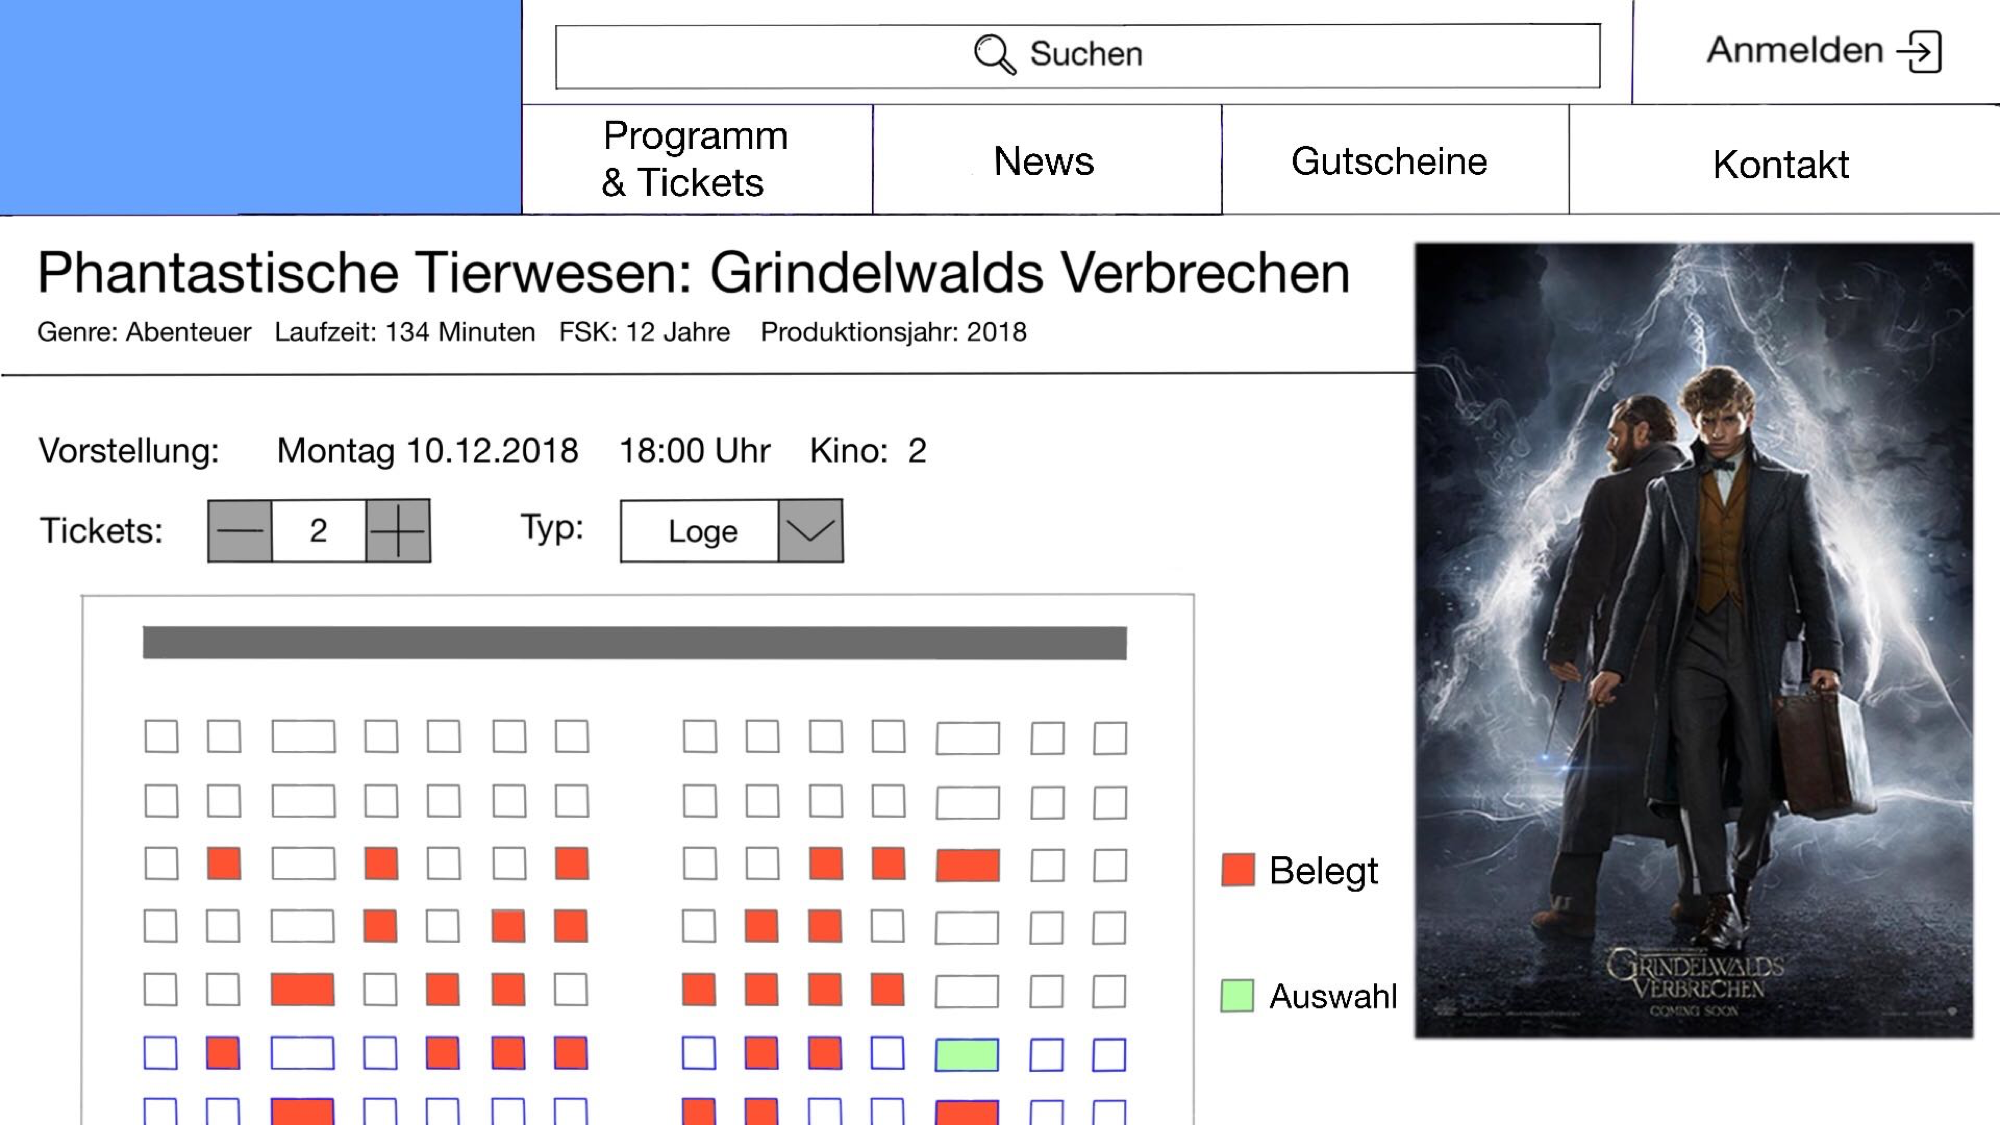
\includegraphics[width=14cm]{img/mockUp3.png}
			\captionsetup{format=hang}
			\caption[Mockup Sitzplan]{\label{fig:mockUpSitzplan} Mockup Sitzplan }
		\end{figure}
	
	\section[Technischer Entwurf]{Technischer Entwurf{\hfill \normalsize Felix Waage}} 	

		Das \ac{ICS} ist ein komplexes Softwaresystem, welches aus verschiedenen Komponenten, Services und Schichten besteht. Aus diesem Grund war es bereits von Beginn an wichtig einen genauen Entwurf der späteren Softwarearchitektur zu entwickeln. Diese Vorgehensweise hat nicht nur den Vorteil, dass Zusammenhänge besser verstanden werden, sondern Probleme auch schneller zu finden und zu beheben sind. Darüber hinaus wird nur so eine effektive und gute Zusammenarbeit zwischen den Teammitgliedern ermöglicht und später die Wartung des gesamten Softwaresystem vereinfacht.
		
		Im weiteren Verlauf dieses Kapitel sollen die verschiedenen Schichten erläutert und deren Kommunikation untereinander beschrieben werden. Des Weiteren wird das Datenbankmodell definiert und näher auf die Architektur des Backends eingegangen.
		
		\subsection{Entwurfsprinzipien}
		Beim Entwurf eines Softwaresystem ist es besonders wichtig konsistent und gründlich zu arbeiten. Dies ist bedingt durch die Tatsache, dass immer mehrere Personen am \ac{ICS} arbeiten und den Entwurf verstehen müssen. Aus diesem Grund wurden vor Beginn der Entwicklung des Entwurfs einige Prinzipien festgelegt. Alle Prinzipien, welche folgend aufgelistet und erläutert werden, sollen unter anderem die Übersichtlichkeit, die Wartbarkeit und die Wiederverwendbarkeit des gesamten Projekts oder von Teilen davon ermöglichen.
		\begin{itemize}
			\item \textbf{Das Prinzip einer einzigen Verantwortung} -- Um die Komplexität und Organisation des Softwareprojekts beherschen zu können, wird das Projekt in verschiedene Module aufgeteilt. Dabei könne einzelene Module wieder aus anderen Modulen zusammen gesetzt sein. Es gilt so Komplexitäten aufzulösen. Jedes Modul übernimmt dabei genau eine Verantwortung und jede Verantwortung wir von genau einem Modul übernommen. Verantwortung ist in diesem Fall die Verpflichtung eine Anforderung umzusetzen. \autocite[Vgl.][]{Lahres.2015}
			\item \textbf{Trennung der Anliegen} -- Jedes Anliegen in einer Anwendung soll durch eigenes Modul realisiert werden. Ein mögliches Anliege wäre zum Beispiel die Transaktionssicherheit, welche unter anderem bei der Reservierung benötigt wird, jedoch auch bei weiteren Anforderung wiederverwendet werden können soll.\autocite[Vgl.][]{Lahres.2015} 
			\item \textbf{Wiederholungen vermeiden} -- Wenn gleiche Funktionalitäten in einem Softwaresystem mehrfach verwendet werden, sollte diese in ein Modul ausgelagert werden, um mögliche Redundanzen zu vermeiden. Dies könnte vor allem dann zum Problem führen, wenn im Code Fehler entdeckt wurden und dieser Fehler so an mehreren Stellen im Quelltext behoben werden muss. Dies stellt eine große Fehlerquelle dar und sollte somit vermieden werden.\autocite[Vgl.][]{Lahres.2015} 
			\item \textbf{Trennung der Schnittstelle von der Implementierung} -- Jedes Modul sollte nur von einer klar definierten Schnittstelle von einem anderen Modul abhängig sein. Dabei spielt die Implementierung der einzelnen Funktionalitäten keine Rolle. Der Quelltext der einzelnen Funktionalitäten soll demnach ausgetauscht werden können, ohne Änderungen an den Schnittstellenaufrufen vornehmen zu müssen. Dies macht das Softwaresystem verständlicher und einfacher zu warten.\autocite[Vgl.][]{Lahres.2015} 
			\item \textbf{Testbarkeit} -- Um direkt während der Entwicklung auf Fehler reagieren zu können ist es wichtig darauf zu achten, dass sich die einzelnen Module und Softwarekomponenten einzelnen Testen lassen. So werden neben der eigentlichen Funktionalität auch Unit-Test implementiert. Dies soll möglichst parallel zur Entwicklung der Funktionalität geschehen und muss beim Erstellen des Entwurfs beachtet werden.\autocite[Vgl.][]{Lahres.2015} 
		\end{itemize} 
		
		Wie in vermutlich jedem großen Softwareprojekt, kann es zu Sonderfällen kommen, wodurch nicht immer alle Prinzipien genau angewendet wurden. Im weiteren Verlauf dieses Kapitel wird an geeigneten Stellen noch einmal auf verschieden Prinzipien verwiesen, um deren Anwendung besser zu erläutern.
		
		\subsection{Schichtenmodell ICS} \label{schichtenmodell}
		
		
		\begin{figure}[H]
			\centering 
			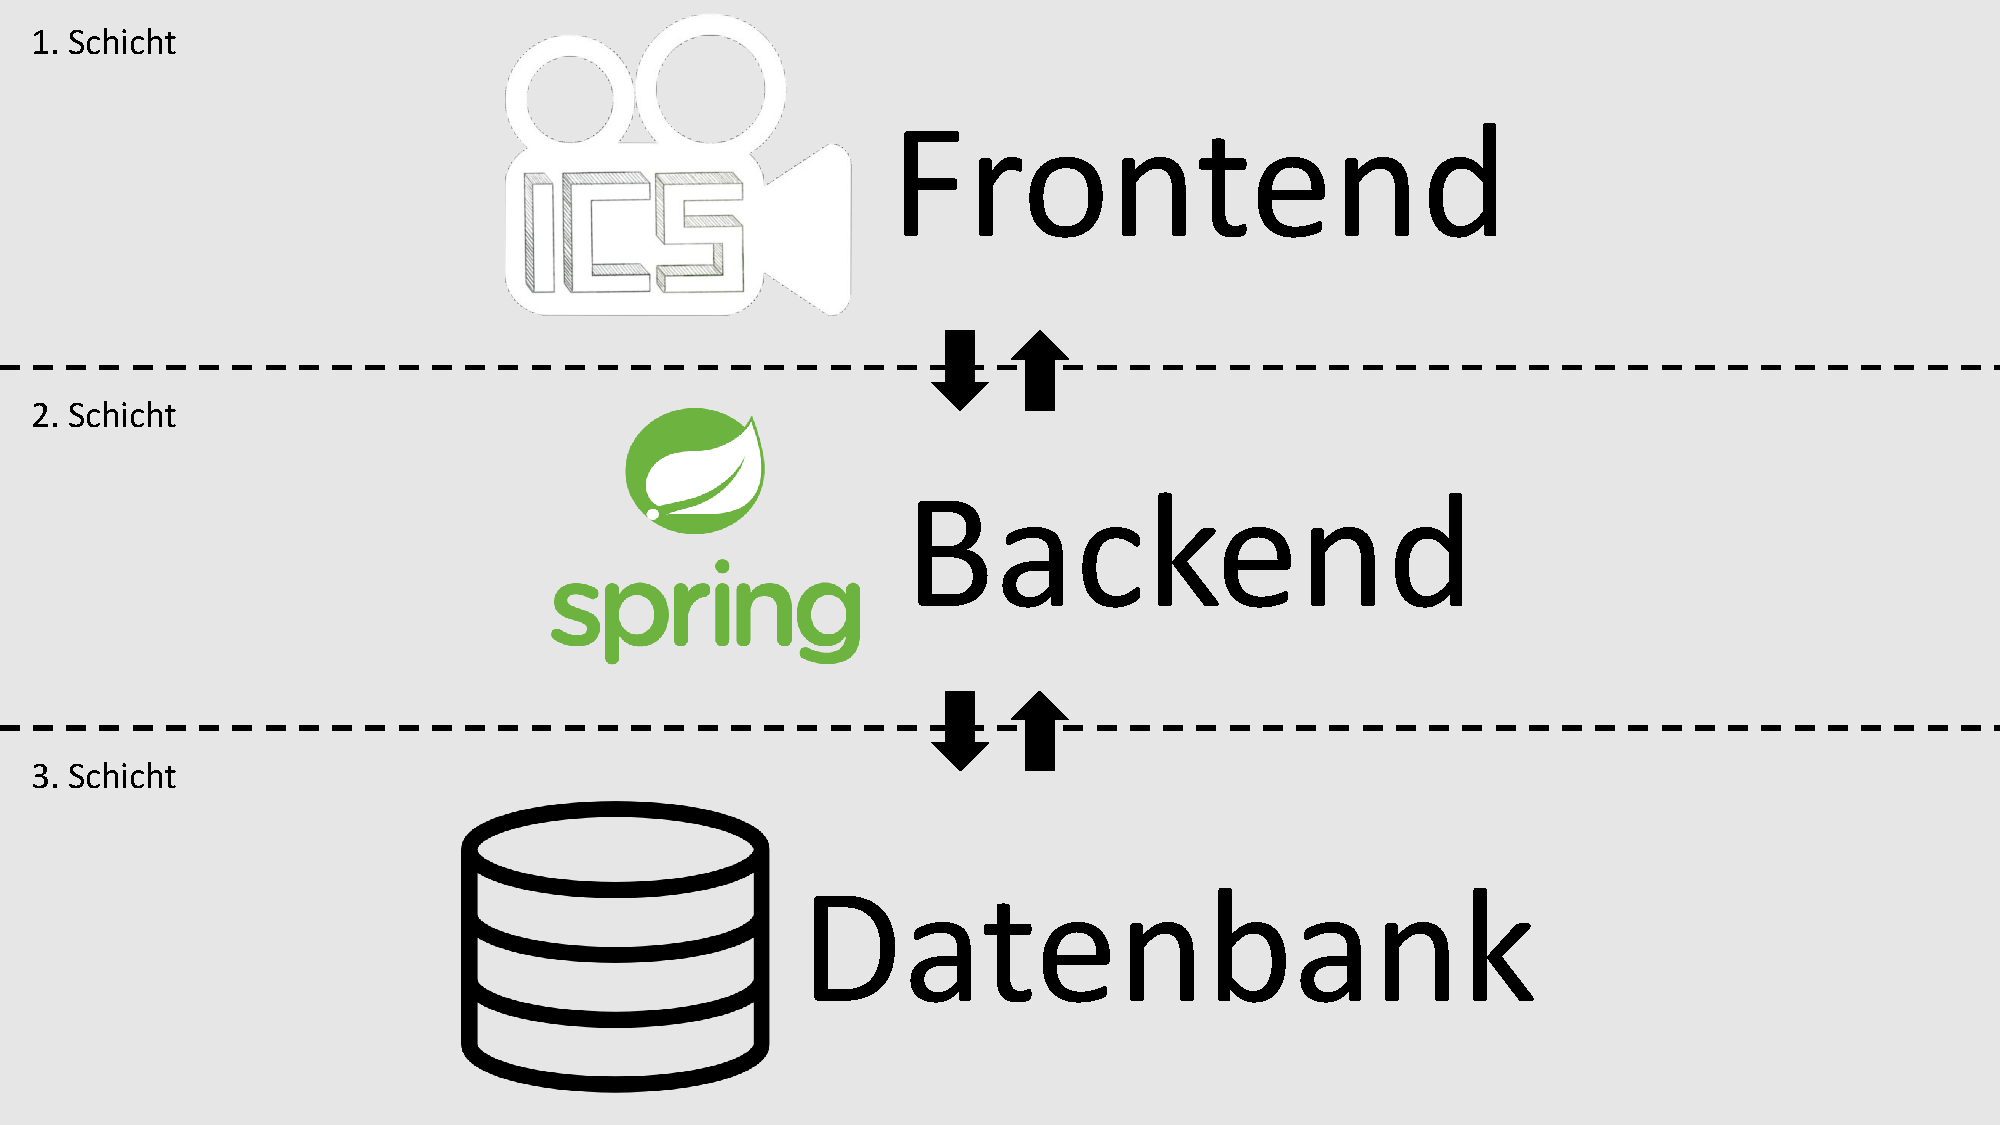
\includegraphics[width=12cm]{img/Schichtenmodell_ICS.pdf}
			\captionsetup{format=hang}
			\caption[Klassendiagramm]{\label{fig:Schichtenmodell} Schichtenmodell des ICS }
		\end{figure}
		
		Die Entwicklung des technischen Entwurfs für das \ac{ICS} wurde damit begonnen die notwendigen Schichten zu identifizieren und in Relation zueinander zu setzen. Es wurde beschlossen das Softwaresystem in drei Schichten aufzutrennen. 
		
		Die oberste Schicht ist das \glqq \textbf{Frontend}\grqq{}, welches die grafische Schnittstelle zum Benutzer darstellt. Über das Frontend kann der Benutzer zum Beispiel Filme suchen, Informationen zu Filmen einsehen und Tickets für eine Vorstellung reservieren. Diese Informationen erhält das Frontend durch HTTP-Request vom Backend.
		
		Im \glqq \textbf{Backend}\grqq{} ist die Fachlogik des Softwaresystem abgebildet, welche zum Beispiel zur Überprüfung der Korrektheit einer Reservierung benötigt wird. Darüber hinaus werden vom Backend die benötigten Restschnittstellen bereitgestellt und die Verbindung zur Datenbank organisiert. 
		
		Die \textbf{Dankbank} dient der Speicherung sämtlicher Daten und Informationen. Sie ist direkt mit dem Backend verbunden und nimmt Anfragen über SQL entgegen. 
		
		Für die Trennung des Softwaresystems in drei Schichten gibt es verschieden Gründe. Zum einen werden für die Implementierung des Frontends andere Technologien verwendet als für das Backend oder der Datenbank. Darüber hinaus verlangen die Anforderungen an das \ac{ICS} eine zentrale Datenhaltung, was sich am besten durch unterschiedliche Schichten realisieren lässt. Darüber hinaus ist es durch die Trennung der Schichten eine einfache Skalierung möglich, falls zum Beispiel mehrere Kino dieses System parallel nutzen möchten.
		\subsection{Entity Relationship Modell}\label{chapter:er-diagramm}
		Resultierend aus den Anforderung an das \ac{ICS} gilt es ein Modell zu entwerfen, welches möglichst genau die spätere Fachlogik repräsentieren kann. Dazu bietet sich für den Anfang das \glqq Entity Relationship Modell\grqq{} an.
		
		Das \textit{\glqq Entity Relationship Modell\grqq{}} ist ein Datenmodell, welches zur Modellierung von logischen Datenbeziehungen verwendet wird. Der Vorteil in der ER-Modellierung liegt in der einfachen Übertragbarkeit in ein logisches relationales Datenbankmodell, dem \textit{Relationenmodell von Codd}. Ein ER-Diagramm nach der Chen-Notation besteht aus Folgenden Bestandteilen:\autocite[Vgl.][]{Stobitzer.0130201914:40Uhr}
		\begin{itemize}
			\item \textbf{Entität/Entität-Typ} -- Unter einer Entität versteht man ein Objekt der realen Welt (Wie z.B.: Avatar, VW Golf, Peter). Gleichartige Entitäten lassen sich anschließend zu einem Entität-Typen zusammenfassen (z.B.: Filme, Autos, Personen).\autocite[Vgl.][]{Stobitzer.0130201914:40Uhr} 
			\item \textbf{Relation} -- Durch die Relation wird die Beziehung zwischen zwei Entitäten beschrieben. So existiert zum Beispiel eine Beziehung zwischen dem Ticket und einer Person. Darüber hinaus ist die Beziehung zwischen zwei oder mehreren Entitäten durch die Kardinalität näher bestimmt. So kann eine Person mehrere Tickets gekauft haben, wobei ein Ticket nur zu einer Person gehört.\autocite[Vgl.][]{Stobitzer.0130201914:40Uhr}
			\item \textbf{Attribut} -- Attribute beschreiben Entitäten näher und enthalten Informationen wie: Name, Alter, Preis
		\end{itemize}
		
		Die zuvor erwähnte Chen-Notation wird folgender Maße grafisch dargestellt. (siehe Abbildung \ref{fig:chennotation})
		\begin{figure}[H]
			\centering 
			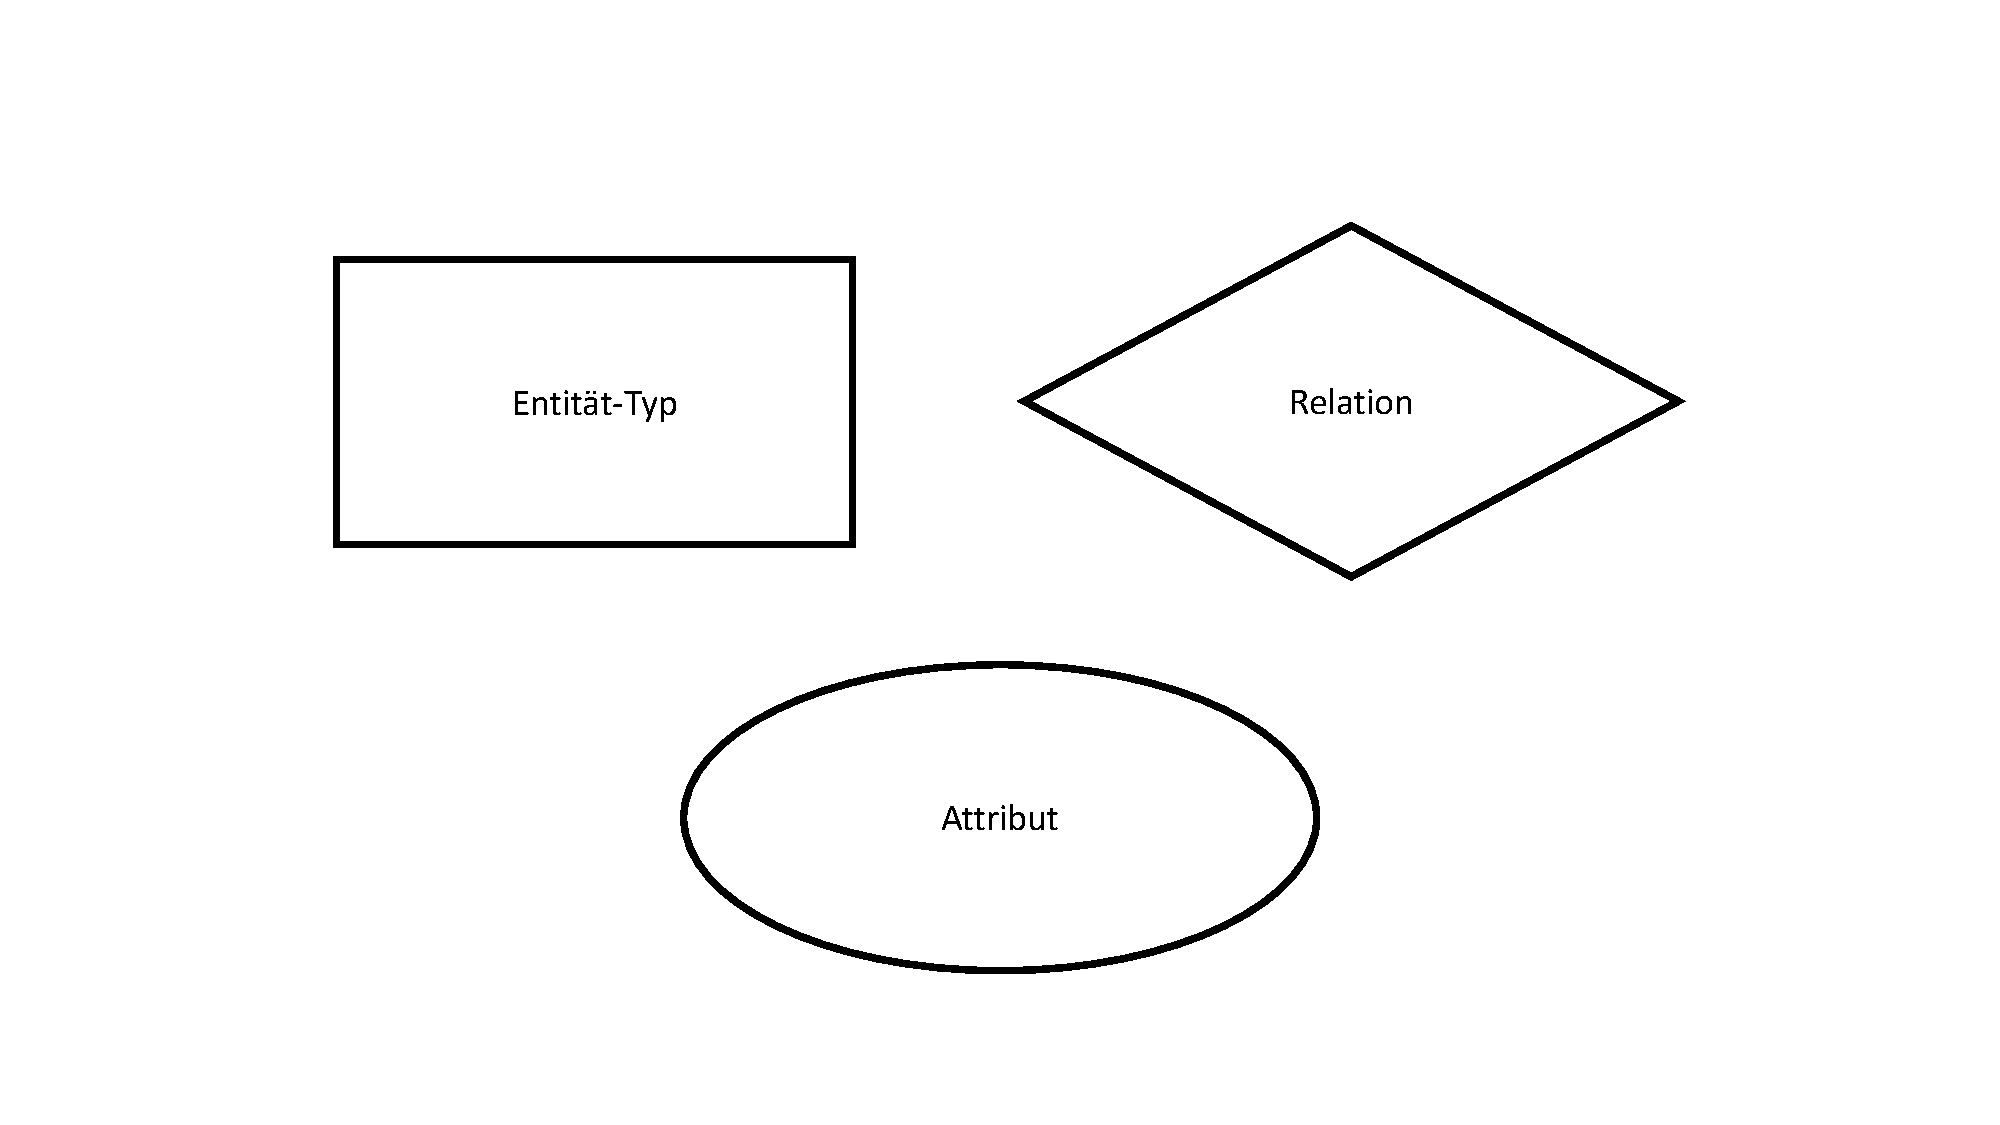
\includegraphics[scale=0.3]{img/ChenNotationERDiagramm.pdf}
			\captionsetup{format=hang}
			\caption[Klassendiagramm]{\label{fig:chennotation} ER-Diagramm nach der Chen-Notation }
		\end{figure}
		
		Unter Nutzung der Anforderung und der Chen-Notation ergibt für das \ac{ICS} das ER-Modell in Abbildung \ref{fig:erModell}.
		
		\begin{figure}[H]
			\centering 
			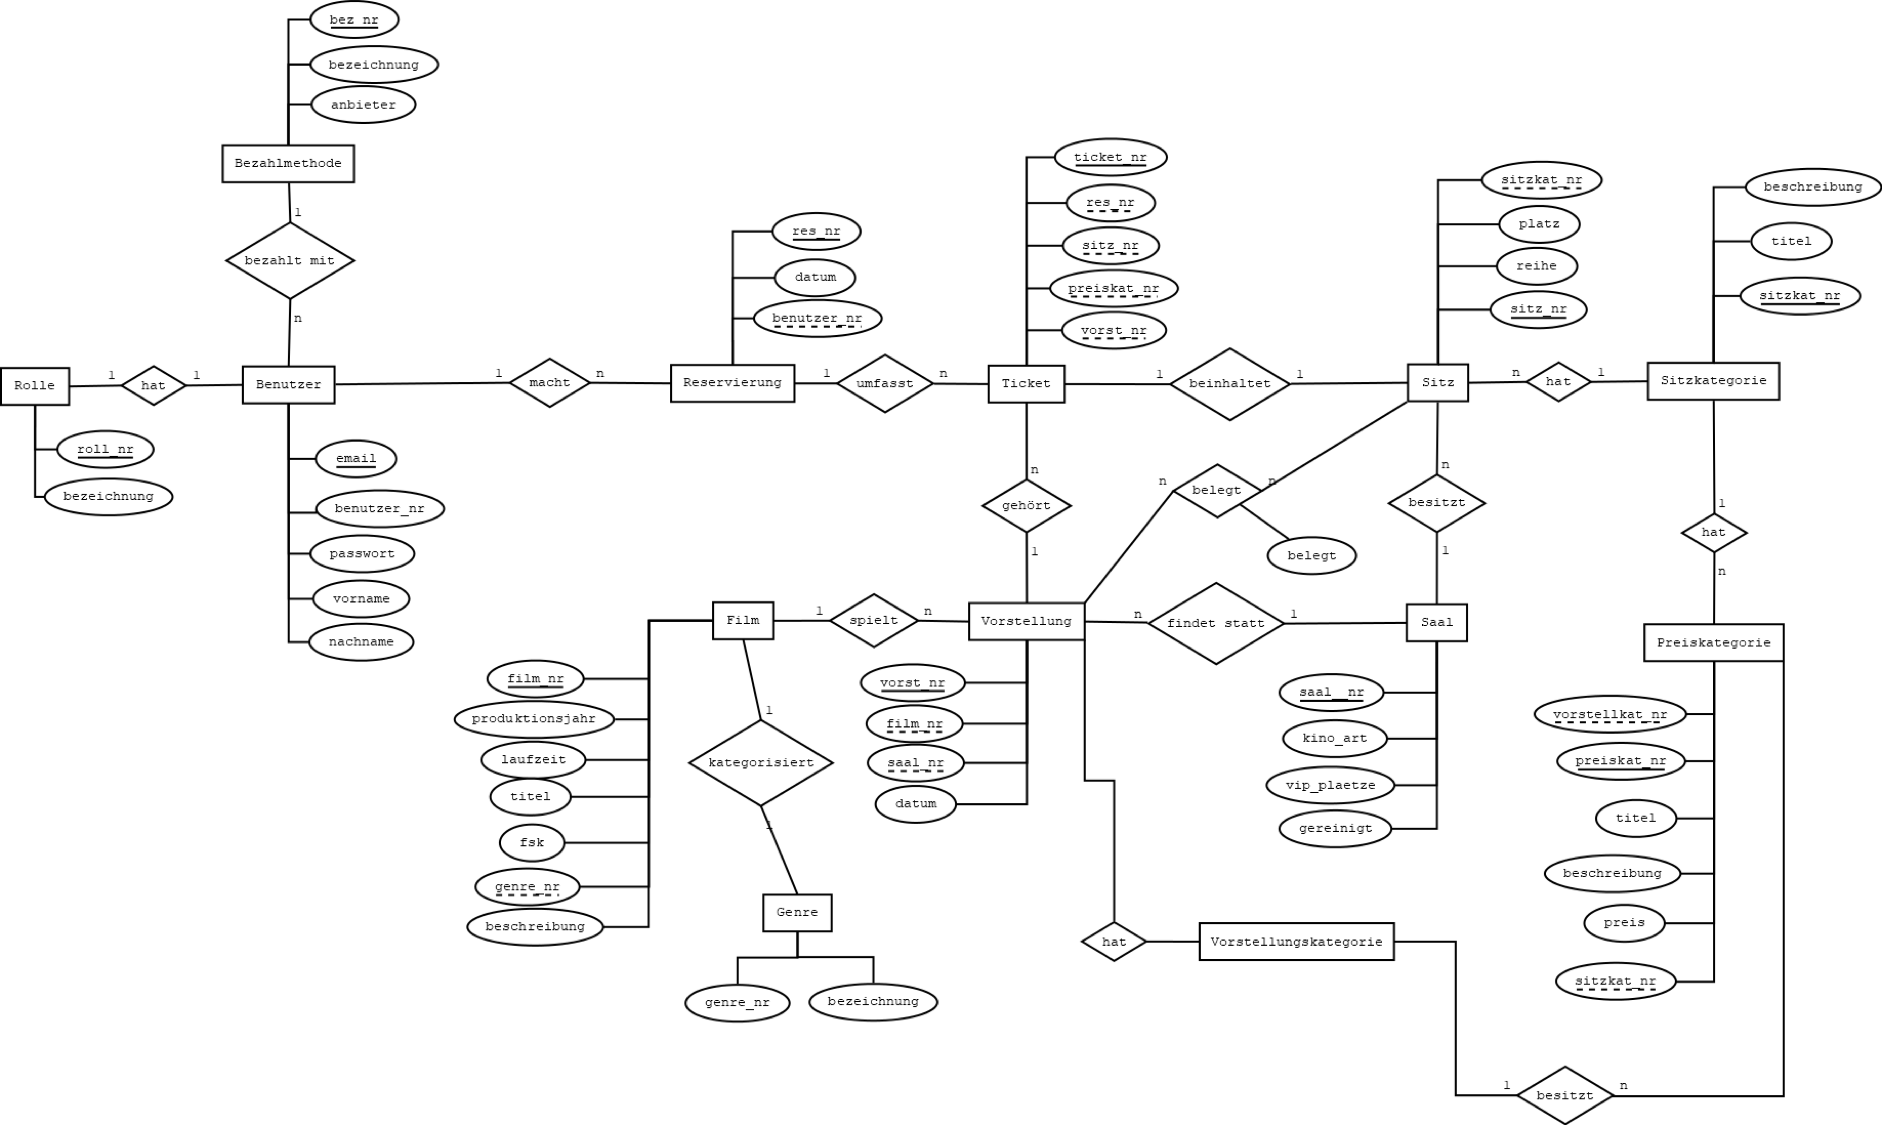
\includegraphics[angle=-90,width=13cm]{img/erModell.png}
			\captionsetup{format=hang}
			\caption[Entity Relationship Datenmodell]{\label{fig:erModell} Entity Relationship Datenmodell}
		\end{figure}
		
		Mit Hilfe des Entity Relationship Modell kann nun die Datenbank angelegt werden. Dazu sind bestimmte Regeln und Vorgehensweisen anzuwenden um die benötigten Tabellen und Spalten aus dem ER-Modell zu extrahieren:
		
		Die Tabellen der Datenbank entsprechen den Entitäten im ER-Modell. Die Attribute werden als Spalten überwiegend unverändert übernommen. Als Schlüssel bietet es nun an ein zusätzliches Schlüsselattribut hinzuzufügen, dieser ist oft eine fortlaufende Nummer oder eine UUID (\textit{Universally Unique Identifier}). Um die Beziehungen zwischen den Attributen richtig abbilden zu können, müssen die Kardinalitäten beachtet werden. 
		\begin{itemize}
			\item 1:1 Beziehung -- Bei dieser Form der Kardinalität enthält eine der beiden Tabellen den Primärschlüssel der anderen Tabelle in Form eines Fremdschlüssels.
			\item 1:n Beziehung -- Liegt diese Form der Kardinalität vor wird der Primärschlüssel der Entität die nur einfach in der Beziehung beteiligt ist als Fremdschlüssel auf der n-Seite hinzugefügt. 
			\item n:m Beziehung -- Sind beide Entitäten in der Beziehung mehrfach beteiligt gilt es eine zusätzliche Tabelle anzulegen. Diese enthält die Primärschlüssel der beteiligten Entitäten als Fremdschlüssel.
		\end{itemize}
		
		\subsection{Klassendiagramm}
		Ein Klassendiagramm dient der strukturierten Darstellung der zu verwenden Klassen, Schnittstellen sowie deren Beziehungen. Das Klassendiagramm ist die Grundlage für die Implementierung des Backends für das \ac{ICS}, da hier Repräsentanten der Entitäten aus Abschnitt \ref{chapter:er-diagramm} in Form von Java-Objekten benötigt werden, um diese später in der Datenbank speichern zu können. Der Entwurf des Klassendiagramms wurde anhand des zuvor erstellten ER-Diagramms angefertigt. Dabei wurde darauf geachtet, das die UML-Notation eingehalten wird.
		
		Eine Klasse repräsentiert eine Gruppe von Objekten mit ähnlichen Eigenschaften. Sie besitzt dazu Funktionen und Attribute, welche die Eigenschaften des jeweiligen Objekts definieren. Die einfachste Form einer Klasse ist die anonyme Klasse. Sie wird in UML wie folgt dargestellt (Abbildung \ref{fig:uml_anonym_class}):
		\begin{figure}[H]
			\centering 
			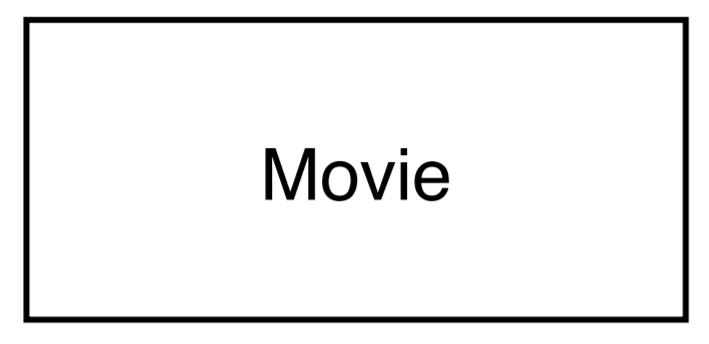
\includegraphics[width=4cm]{img/uml_anonym_class.JPG}
			\captionsetup{format=hang}
			\caption[Anonyme Klasse in UML-Notation]{\label{fig:uml_anonym_class}Anonyme Klasse in UML-Notation}
		\end{figure}
		Diese Darstellung kann durch Attribute und Funktionen erweitert werden, wobei die Sichtbarkeit der Attribute und Funktionen bereits im Klassendiagramm beschrieben werden sollte. In Java sind drei Zugriffsmodifikatoren definiert:
		\begin{itemize}
			\item\textbf{public} -- Es kann von Außen auf das Attribut oder die Funktion direkt zugegriffen werden. Dies kann dazu führen, dass Klassenbestandteile nicht sinngemäß verwendet werden. In UML wird dieser Zugriffsmodifikator durch ein + vor dem Attribut oder der Funktion dargestellt. 
			\item\textbf{private} -- Nur Funktionen innerhalb der Klasse können auf diese Attribute oder Funktionen zugreifen. Die Notation UML beschreibt dies mit einem - vor dem Attribut oder der Funktion.
			\item\textbf{protected} -- Durch den Zugriffmodifikator protected ist es auch Subklassen mögliche, auf Attribute und Funktionen zuzugreifen. In der UML-Notation wird dieser Zugriffsmodifikator durch \# repräsentiert.
		\end{itemize}
		Allgemein ist es jedoch üblich Attribute grundsätzlich als \texttt{private} zu deklarieren und den Zugriff durch sogenannte \textit{Getter- und Setter-Methoden} zu ermöglichen. Dies ermöglicht es Werte vor dem Speichern auf Korrektheit zu prüfen. Außerdem kann so ein Missbrauch der Klasse für andere Zwecke verhindert werden. Eine Klasse mit all den erwähnten Bestandteilen wird in UML wie folgt dargestellt (Abbildung \ref{fig:KlasseUML}): 
		\begin{figure}[H]
			\centering 
			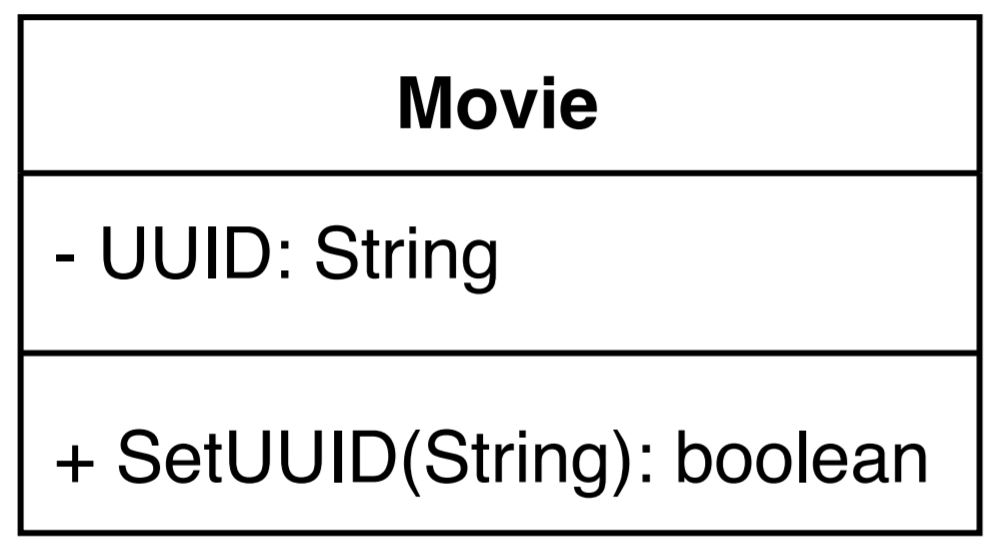
\includegraphics[width=4cm]{img/uml_class.JPG}
			\captionsetup{format=hang}
			\caption[Klasse in UML-Notation]{\label{fig:KlasseUML}Klasse nach der UML-Notation}
		\end{figure}
		Die Relationen zwischen den Klassen, werden durch Pfeile und Linien visualisiert, welche wie beim ER-Diagramm an den Enden die Kardinalität der Beziehung angeben. 
		
		\begin{figure}[H]
			\centering 
			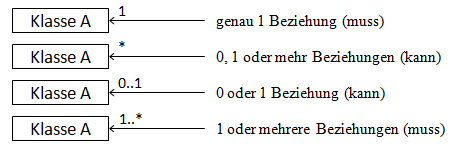
\includegraphics[width=15cm]{img/UmlKardinalitaet.png}
			\captionsetup{format=hang}
			\centering\caption[Kardinalitäten nach UML-Notation]{\label{fig:Kardinalitaeten.UML}Startseite von Kinopolis\footnotemark}
		\end{figure}\footnotetext{Quelle: http://www.info-wsf.de/index.php/Assoziationen\_und\_Kardinalit\%C3\%A4ten}
		
		Neben den Kardinalitäten werden auch Aggregationen und Kompositionen in der UML-Darstellung ermöglicht. Eine \textit{Aggregation} ist eine besondere Form der Beziehung zwischen zwei Klassen. Sie drückt aus, das eine Klasse aus anderen Klassen besteht. Verbal wird dies oft mit \textit{besteht aus, hat, ist Bestandteil von} ausgedrückt. Eine Komposition ist ähnlich zur Aggregation mit dem Unterschied das die Existenz der einen Klasse von der anderen abhängt. So kann zum Beispiel ein Raum nicht ohne ein Gebäude existieren. In UML wird dies wie folgt dargestellt:
		
		\begin{figure}[H]
			\centering 
			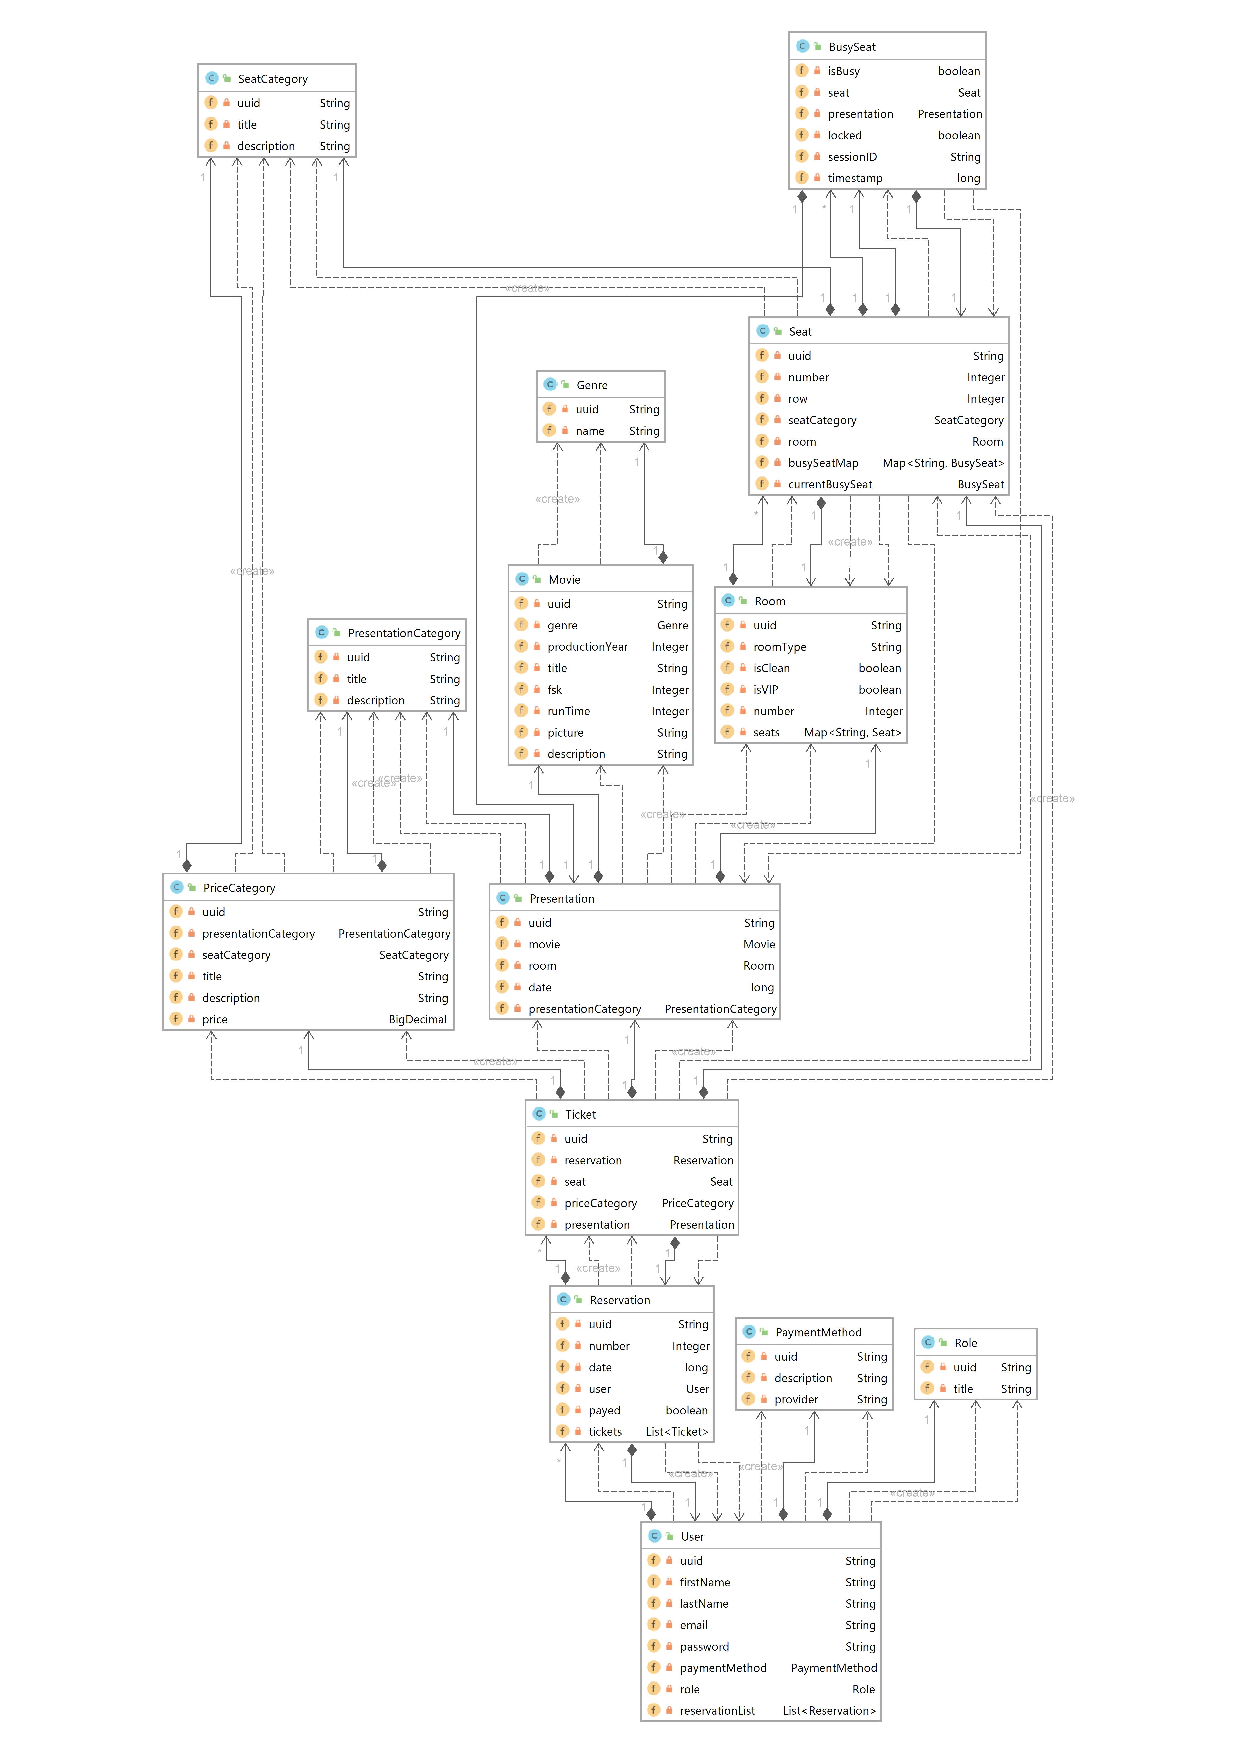
\includegraphics[width=15cm]{img/class_diagramm.pdf}
			\captionsetup{format=hang}
			\caption[Klassendiagramm]{\label{fig:Klassendiagramm}Klassendiagramm}
		\end{figure}
		
		\subsection{Dynamische Modelle}
		\begin{figure}[H]
			\centering 
			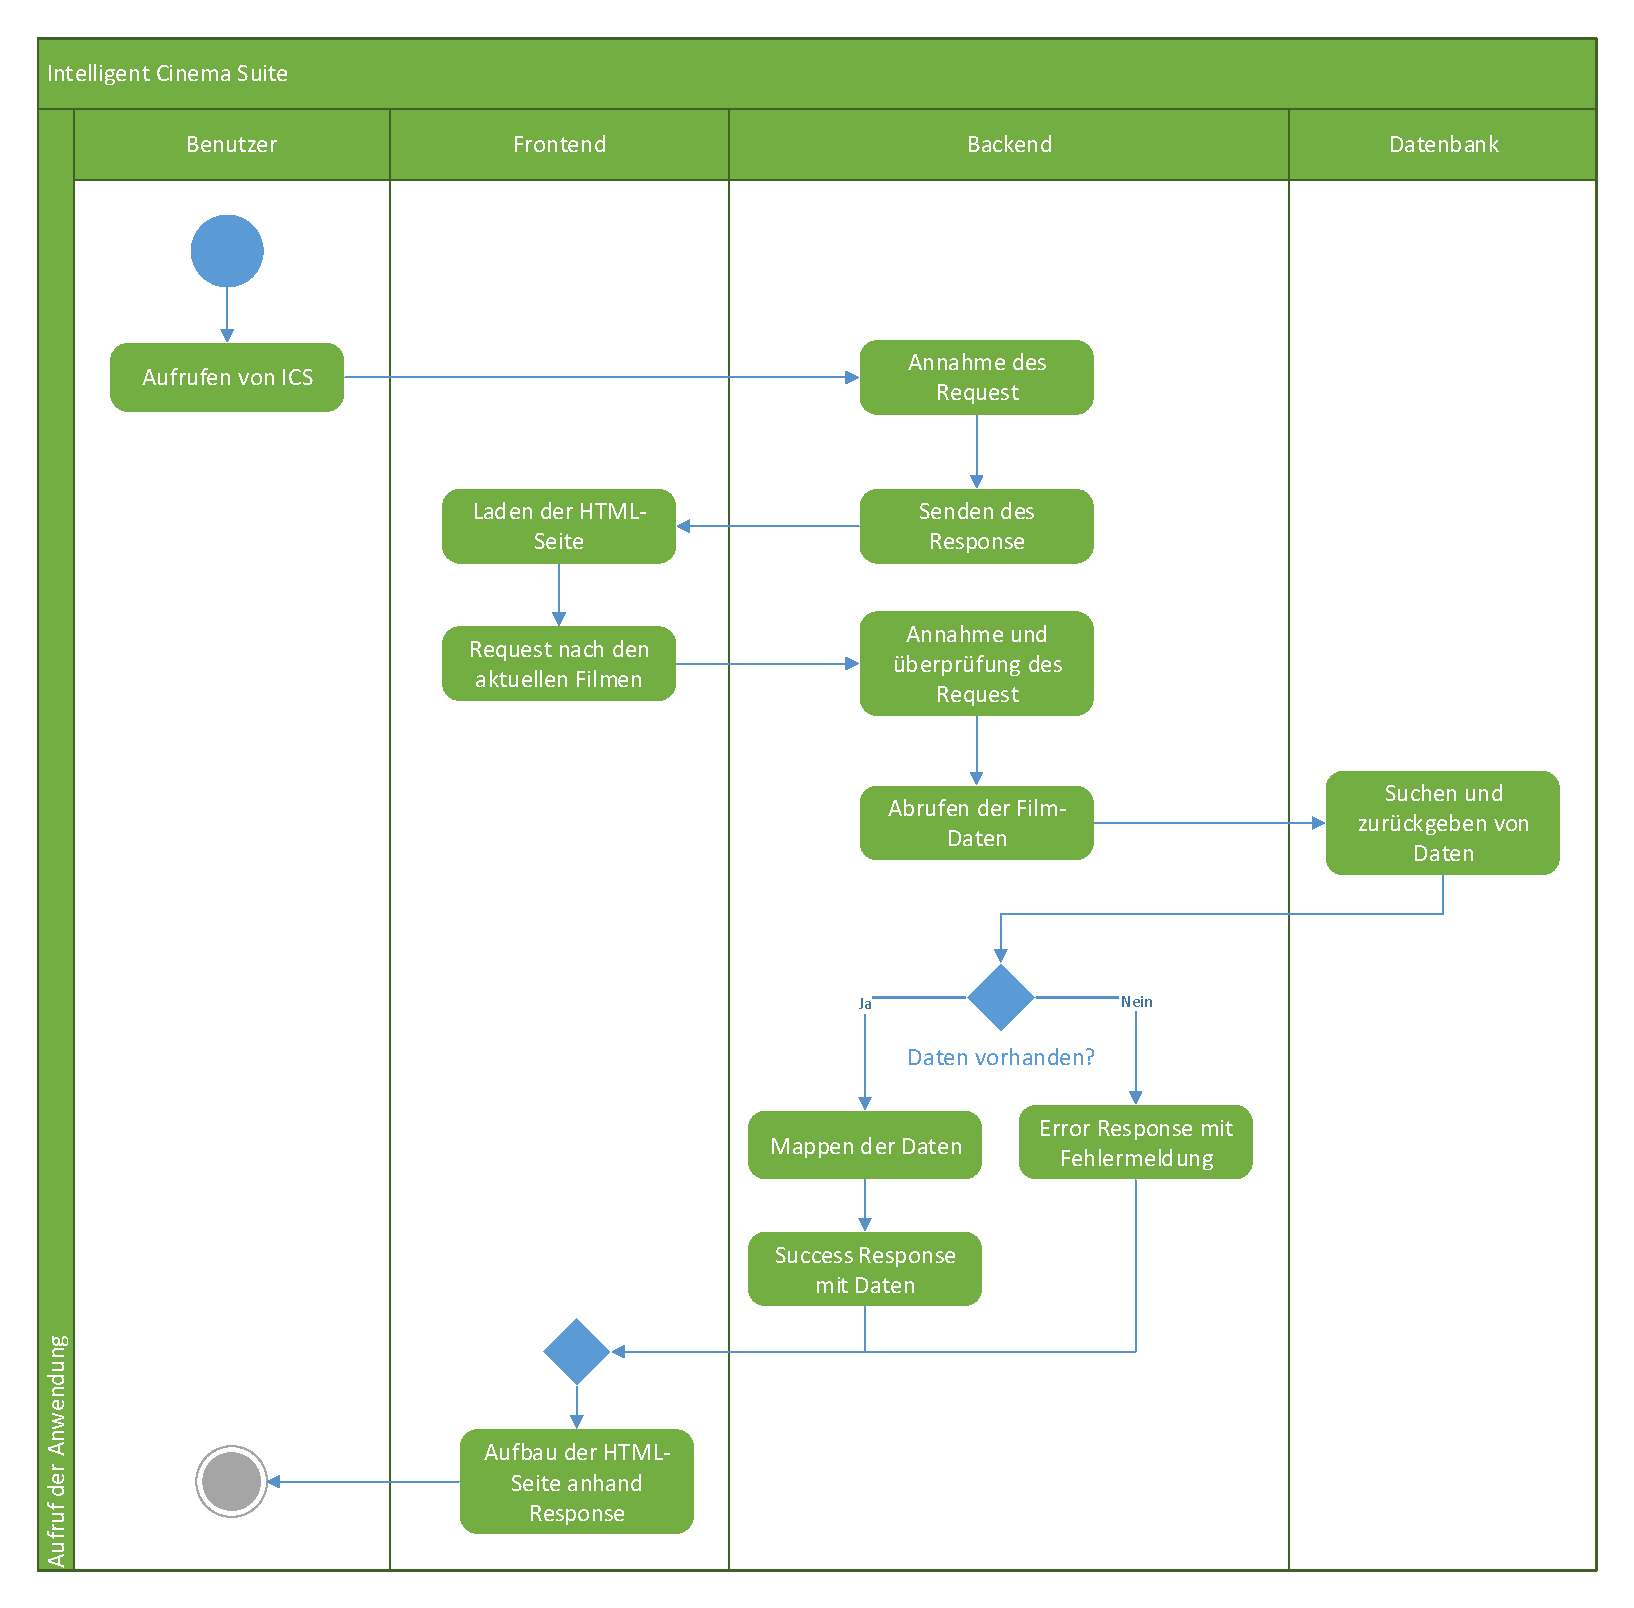
\includegraphics[width=15cm]{img/adSeitenaufruf.pdf}
			\captionsetup{format=hang}
			\caption[Aktivitätsdiagramm Seitenaufruf]{\label{fig:aktivitätSeitenaufruf}}
		\end{figure}
		
		%           \begin{figure}[H]
		%               \centering 
		%               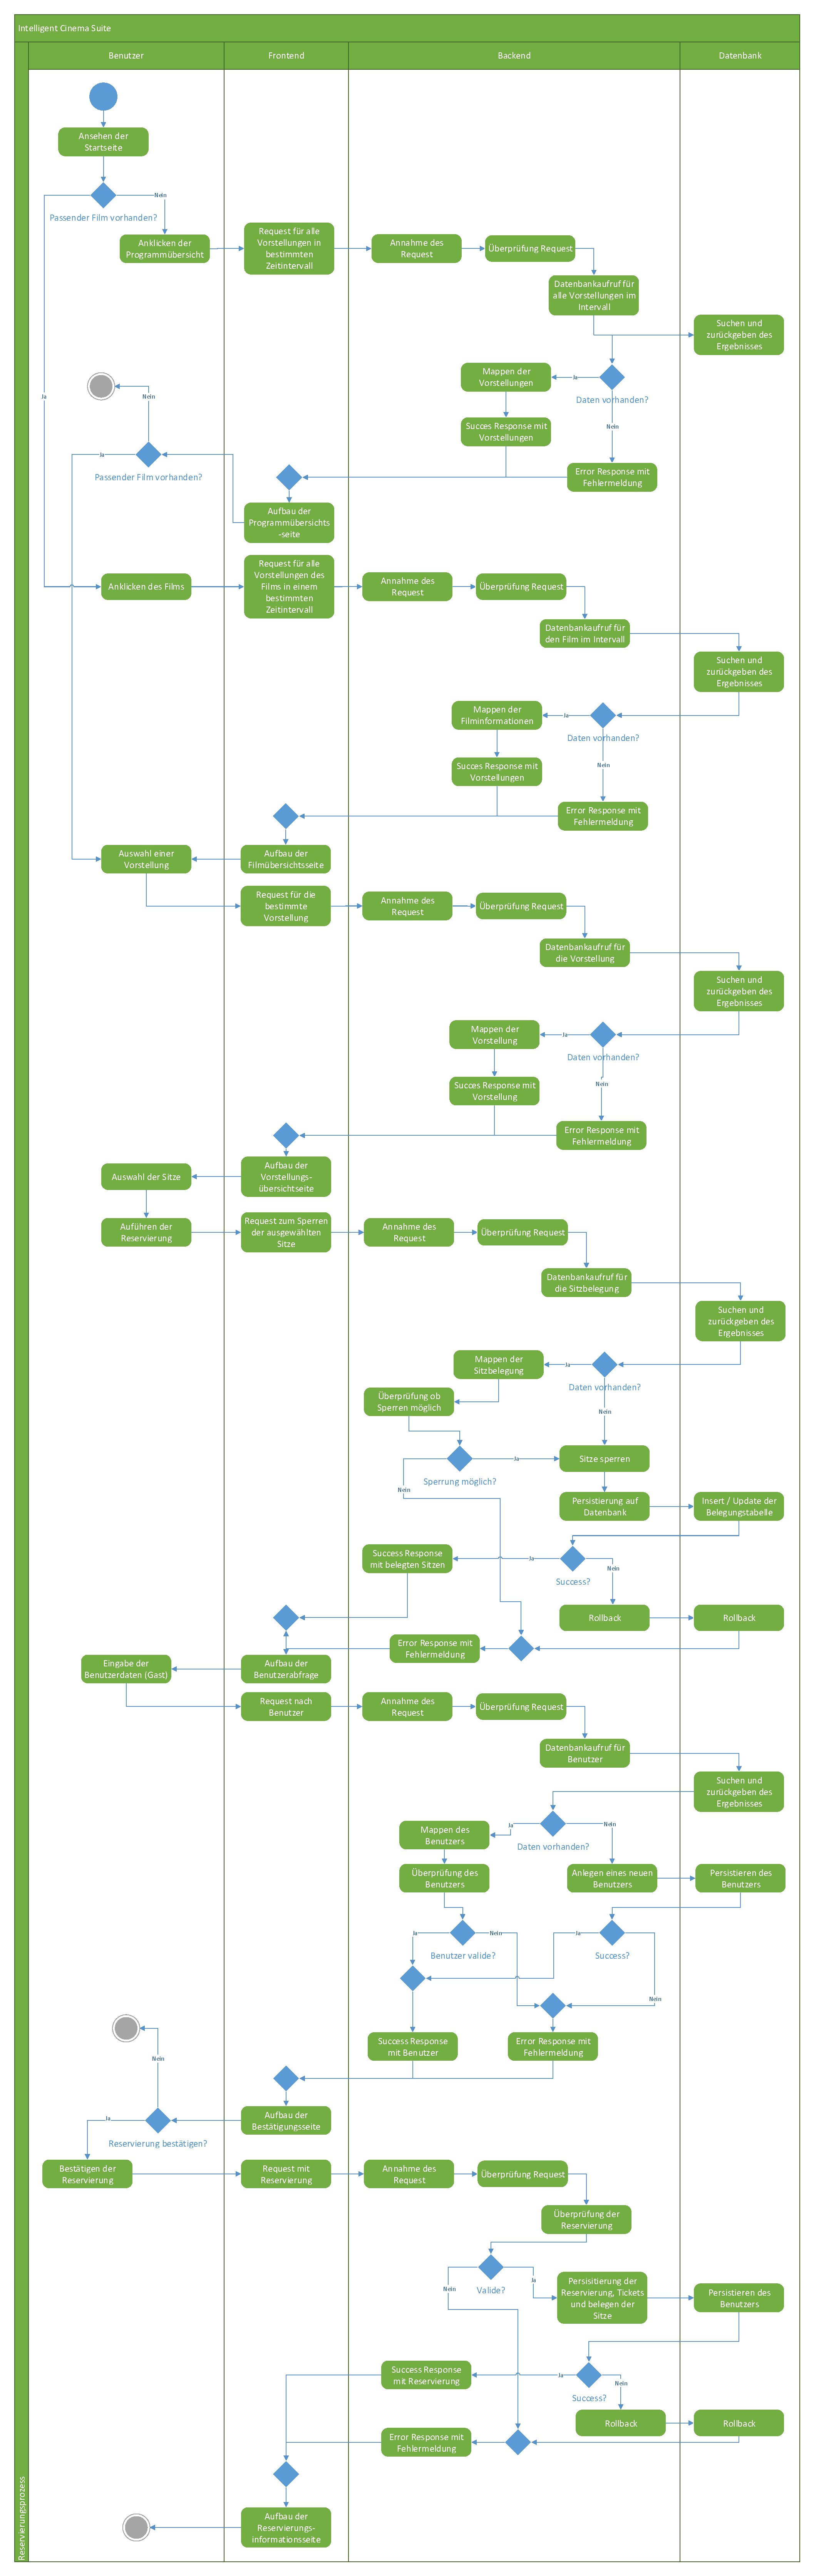
\includegraphics[width=14cm]{img/adReservierung.pdf}
		%               \captionsetup{format=hang}
		%               \caption[Aktivitätsdiagramm Seitenaufruf]{\label{fig:aktivitätSeitenaufruf} Aktivitätsdiagramm Reservierung}
		%           \end{figure}